\begin{frame}[t]{BERT \& XLM-RoBERTa: encoder làm reward model}
  \begin{columns}[T,onlytextwidth]
    \begin{column}{0.46\textwidth}
      \begin{block}{XLM-RoBERTa làm Reward Model}
        \small
        \begin{itemize}
          \item Phiên bản BERT đa ngôn ngữ (100+ ngôn ngữ, kể cả \textbf{tiếng Việt})
          \item Fine-tune trên tập \textit{Dining Review} theo tiêu chí \textbf{engagement}
          \item Cho điểm $r$ mỗi câu trả lời $\rightarrow$ tín hiệu huấn luyện cho \textbf{GRPO}
          \item Hiệu quả khi tập train và tập áp dụng \textit{cùng miền}
        \end{itemize}
      \end{block}
      \vfill
      {\scriptsize\itshape Kết quả thực tế của reward model này sẽ được phân tích trong phần thực nghiệm.}
    \end{column}
    \begin{column}{0.50\textwidth}
      \centering
      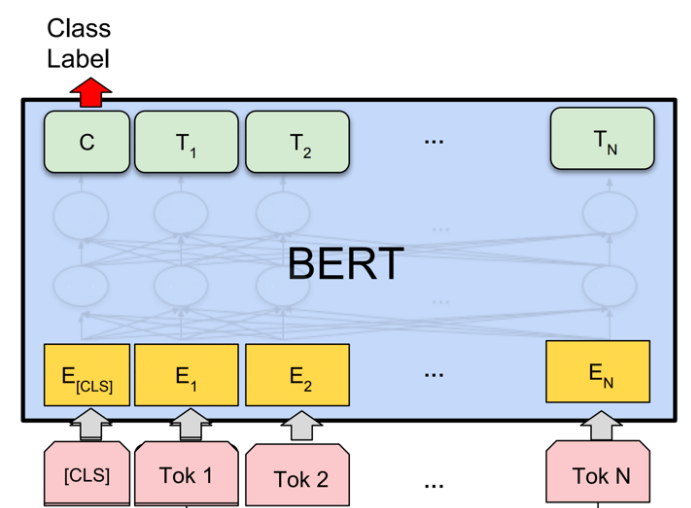
\includegraphics[width=\linewidth]{images/BERT.png}\\[0.4em]
      {\scriptsize Kiến trúc BERT: token \texttt{[CLS]} được dùng để tổng hợp
       biểu diễn toàn câu, sau đó qua một linear layer cho ra điểm reward.}
    \end{column}
  \end{columns}
\end{frame}
